\chapter{Android Development}

Android offers a software stack for mobile devices. Apart from what people refer to as the Operation System, it also contains middleware and key applications. The Android SDK offers the necessary tools and APIs to start developing Android applications. These applications are developed using the Java programming language. The following are the most important features of the Android stack:

\begin{itemize}
\item{\textbf{Application framework} enabling reuse and replacement of components}
\item{\textbf{Dalvik virtual machine} optimized for mobile devices}
\item{\textbf{SQLite} for structured data storage}
\item{\textbf{Media support} for common audio, video, and still image formats (MPEG4, H.264, MP3, AAC, AMR, JPG, PNG, GIF)}
\item{\textbf{GSM Telephony} (hardware dependent)}
\item{\textbf{Bluetooth, EDGE, 3G, and WiFi} (hardware dependent)}
\item{\textbf{Camera, GPS, compass, and accelerometer} (hardware dependent)}
\item{\textbf{Rich development environment} including a device emulator, tools for debugging, memory and performance profiling, and a plugin for the Eclipse IDE}
\end{itemize}

\section{Android Architecture}

This section will explain the major components of the Android architecture. The complete architecture is depicted in figure ~\ref{fig:android_architecture}. We will follow a top-down approach, starting with the lowest level of abstraction (Applications) first all the way down to the Linux Kernel, that provides core system services such as security and memory management.

\begin{figure}[h!]
\centering
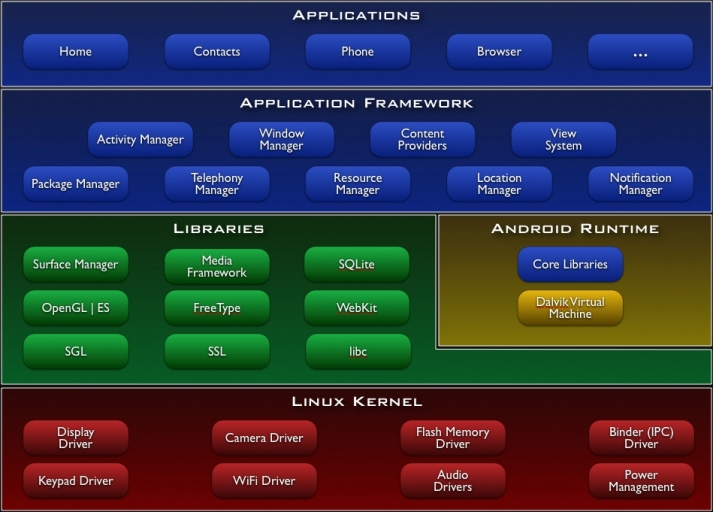
\includegraphics[width=1.0\textwidth]{images/chap4_android_architecture.jpg}
\caption{Android Architecture.}
\label{fig:android_architecture}
\end{figure}

\subsection{Applications}

Android applications are developed using the Java programming language. By default, Android ships with a number of default applications written in Java. These include an email client, SMS program, calendar, maps, browser, contacts and others. In the next section, we will see the major components of a typical Android application. In other words, the building blocks of a minimal Android application.

\subsection{Application Framework}

Android offers the ability to build extremely rich and innovative applications. Developers are granted the same access to the framework APIs used to build the core applications on the top level. The application architecture is designed to simplify the reuse of components; any application can publish its capabilities and any other application may then make use of those capabilities \cite{WhatAndroid}. 
\\ \\
Underlying all applications is a set of systems and services:

\begin{itemize}
\item{A set of \texttt{Views} to build the front-end of the application, including lists, grids, text boxes and buttons. A subset of these Views will be supported on the modeling framework.}
\item{\texttt{Content providers} that manage access to a structured set of data. They encapsulate the data, and provide mechanisms for defining data security. Content providers are the standard interface that connects data in one process with code running in another process. \cite{ContentProviders}}
\item{\texttt{Resource Manager} that provides access to non-code resources such as images and strings, so they can be maintained independently.  Externalizing your resources also allows you to provide alternative resources that support specific device configurations such as different languages or screen sizes, which becomes increasingly important as more Android-powered devices become available with different configurations. \cite{AppResources}}
\item{\texttt{Notification Manager} that notifies the user of events that happen. It allows a developer to tell the user that something has happened in the background \cite{NotificationManager}. For instance, the receival of an SMS can trigger a notification.}
\item{\texttt{Activity Manager} manages the lifecycle of one Activity. More details on Activities and the management can be found in the next section.}
\end{itemize}

\subsection{Libraries}

Although the Android SDK is offered in the Java programming language, the lower level libraries are a set of C/C++ libraries used by various components in the Android system. Like in a typical stacked architecture, a lower level layer is exposed through a higher level layer. Therefore, these libraries are accessible through the Android application framework. Some of the core libraries \cite{WhatAndroid}:

\begin{itemize}
\item{\textbf{System C library} - a BSD-derived implementation of the standard C system library (libc), tuned for embedded Linux-based devices}
\item{\textbf{LibWebCore} - a modern web browser engine which powers both the Android browser and an embeddable web view}
\item{\textbf{SGL} - the underlying 2D graphics engine}
\item{\textbf{SQLite} - a powerful and lightweight relational database engine available to all applications}
\end{itemize} 

\subsection{Android Runtime}

As seen in the above layers, Android has quite a unique application component architecture. In order to make the Android environment suitable for multiple applications, Android executes multiple instances of its own customized Virtual Machine, Dalvik. Basically, each Android application runs in its own process, with its own instance of the Dalvik Virtual Machine. 
\\ \\
As a result of this approach to multiprocessing, Android must efficiently divide memory into multiple heaps, where each heap is as small as possible, so that many applications can fit in memory at the same time. In order to be space-efficient, Android uses a special component lifecycle, which enables objects to be garbage-collected and recreated. Next to this, Dalvik is able to run a bytecode system specifically developed for Android, called dex. Dex bytecodes are approximately twice as space-efficient as Java bytecodes, halving the memory overhead of Java classes for each process.

\subsection{Linux Kernel}

Finally, Android relies on a linux kernel for core system services such as security, memory management, process management, network stack, etc. This kernel also acts as an abstraction layer between the hardware and the rest of the software stack. It controls the hardware elements throughout the software stack and serves as a gateway.

\section{Android Components}

This section will describe the different Android components and their respective managers in depth. We will start with a comparison of traditional versus Android programming. While every Android application is developed in the Java programming language, the approach of writing such an application is different from writing traditional (desktop) applications.

\subsection{Traditional versus Android programming}

When starting applications in a traditional Operating System, there usually exists a single point of entry called \texttt{main}. The OS will load the program code into a process and starts executing it. Additionally, if we look at programs written in Java, it gets a little more complex. A Java virtual machine (JVM) that resides within a process loads bytecode to instantiate Java classes as the program uses them. This process is depicted in figure ~\ref{fig:java_app}.
\\ \\
\begin{figure}[h!]
\centering
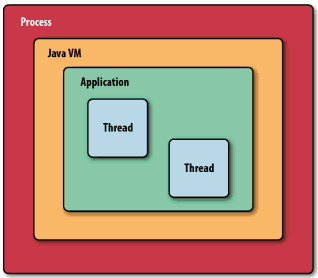
\includegraphics[width=0.5\textwidth]{images/chap4_java_app.png}
\caption{A Java application running in a JVM.}
\label{fig:java_app}
\end{figure}
The Android system works a little different and supports multiple application entry points. Instead of a sequential code hierarchy, an Android program is a cooperating group of components that may be started from outside the normal flow of the application. For example, if your application starts the activity in the camera application that captures a photo, that activity runs in the process that belongs to the camera application, not in your application's process. The photo capture function can be integrated by many applications in their UI flow.

\subsection{Activities and Intents}

Typically, an Android activity is a unit of interaction. It usually fills the whole screen of an Android mobile device. It also functions as a unit of execution. Note that an Android application does not have a single point of entry; an application can have entry points to multiple activities. They are the reusable, interchangeable parts of the flow of UI components across Android applications. An activity interacts with the Android runtime to implement key aspects of the application life cycle.
\\ \\
Now if one activity invokes another, we usually want to pass some information to it. The unit of communication is called Intent. They are the basis of a system of loose coupling that allows activities to launch one another. It is usually a bad idea to keep references to activities in memory, because of the way Android does garbage collection and the restrictions of memory on a mobile device. In general, an activity is an isolated and independent object that only communicates with other activities through intents.

\subsection{Tasks}

So communication in an Android application is defined by means of an intent. Unlike in traditional desktop applications, the UI flow in Android applications is also described through intents. Using these intents, an Android developer can create a chain of activities that spans more than one application. This is referred to as a \texttt{task}. An example of a task spanning multiple activities is depicted in figure ~\ref{fig:android_task}.

\begin{figure}[h!]
\centering
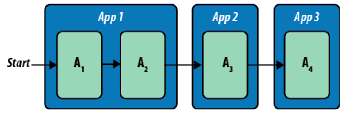
\includegraphics[width=0.7\textwidth]{images/chap4_android_task.png}
\caption{Activities in a single task spanning multiple applications.}
\label{fig:android_task}
\end{figure}

An example of this task can be found in table ~\ref{tab:table1}. In this example, app 1 represents the Android Messaging app. First, a user views all messages and after that decides to read a specific message. These two actions map onto two activities. Afterwards, he decides to view the contact, and the user is sent to another application (and another Activity). When the user decides to call this contact, we need another application again. This one task thus involved three applications and four activities. The UI flow in this task is completely defined by means of intents.

\begin{table}[h!p!]
\caption{A single task across multiple applications and spanning multiple activities}
\begin{tabular}{| l l l |}
\hline
App & Activity & User's next action \\
\hline
Messaging & View list of messages & User taps on a message in the list \\
Messaging & View a specific message & User taps Menu - View Contact \\
Contacts & View a contact & User taps Call Mobile \\
Phone & Call the contact's mobile number & nothing \\
\hline  
\end{tabular}
\label{tab:table1}
\end{table}

\subsection{Other components}

Apart from the \texttt{Activity} class, there are three other important components that contribute to Android applications: services, content providers and broadcast receivers. 
\\ \\
A \texttt{Service} class supports long-running background tasks. They may be active, but not visible on the screen. A typical application that may contain a \texttt{Service} class is a music player. We usually want to continue listening to music while doing some other task.
\\ \\
Next, a \texttt{ContentProvider} class provides access to a data store for multiple applications. An Android developer specifies a special URI starting with \texttt{content://} that gives access to the data store. A \texttt{ContentProvider} class works analogous to a RESTful web service. They have a specific URI and associated operations such as putting and getting data.
\\ \\
Finally, the \texttt{BroadcastReceiver} class allows multiple objects to listen for intents broadcast by applications. \texttt{BroadcastReceiver} is similar to \texttt{Activity}, but does not have its own user interface. 
\\ \\
While these components can possibly be important in Android applications, currently only the \texttt{Activity} class will be supported in our modeling framework. The other components can additionally be implemented as future work.

\subsection{AndroidManifest}

In order for an Android application to know what its contents are, we need to explicitly describe them in an XML file called \textit{AndroidManifest.xml}. In this file, we declare all our activities, services, content providers and broadcast receivers along with their intents. Since an Android application does not have a single point of entry, we also need to specify which component is the main component (also done through another \texttt{Intent}). A visualization of the structure of the AndroidManifest can be found in figure ~\ref{fig:android_manifest}.

\begin{figure}[h!]
\centering
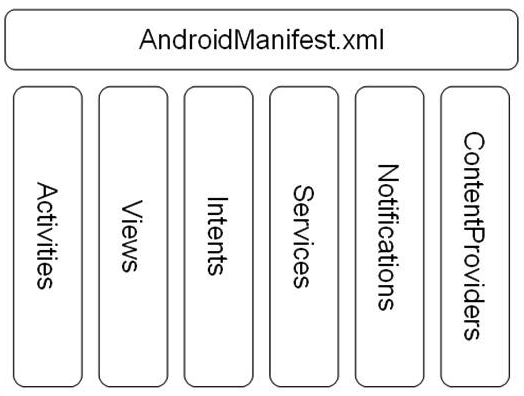
\includegraphics[width=0.7\textwidth]{images/chap4_android_manifest.png}
\caption{Structure of an AndroidManifest.xml.}
\label{fig:android_manifest}
\end{figure}

\subsection{Activity Lifecycle}

As explained earlier, the Android system can enable objects to be garbage collected and recreated. Due to this mechanism activities have a special customized life cycle, because they can easily be garbage collected when inactive. When a user wants to activate the activity again, the Android system will need to be able to recreate the \texttt{Activity} object. Activities are saved on an \textit{activity stack}. The \texttt{Activity} on top of the stack is always the running activity. Activities on the stack below the current one are always invisible and inactive. An activity can be in one of four states:

\begin{itemize}
\item{\textit{Active} or \textit{Running} if the activity is in the foreground of the screen}
\item{\textit{Paused} if the activity has lost focus but is still visible. This activity is still alive but can be killed by the Android system in case of low memory.}
\item{\textit{Stopped} if the activity is obscured by another activity. All state information is still in memory, but the activity is not visible and will most likely be killed when memory is needed elsewhere.}
\item{When the activity is \textit{paused} or \textit{stopped}, the system can ask to finish it or simply kill its process. When a user requests access to the activity again, it should be restored to its previous state.}
\end{itemize}

In figure ~\ref{fig:activity_lifecycle}, the important states of an Activity lifecycle are visualized. The states an Activity can be in are the colored ovals. The rectangles introduce the callbacks a developer can implement to perform operations when moving between states.

\begin{figure}[h!]
\centering
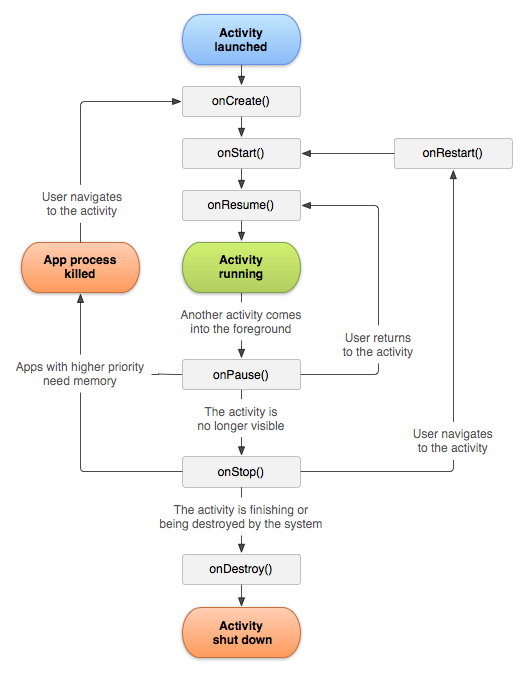
\includegraphics[width=0.9\textwidth]{images/chap4_activity_lifecycle.png}
\caption{The lifecycle of an Android Activity.}
\label{fig:activity_lifecycle}
\end{figure}

\section{Android App Inventor}

Android App Inventor is an application provided by Google that allows anyone to create applications for the Android system. Google wanted to encourage people to create software for the Android platform, even people unfamiliar with computer programming. App Inventor provides a graphical interface that has drag-and-drop functionality, so that users can easily create new applications or prototypes. An example of the application is depicted in figure ~\ref{fig:app_inventor}.

\begin{figure}[h!]
\centering
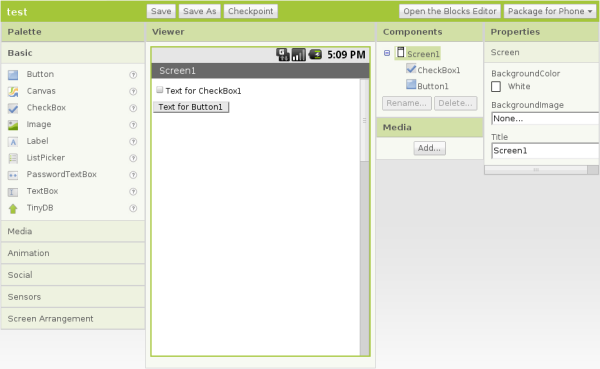
\includegraphics[width=1.0\textwidth]{images/chap4_app_inventor.png}
\caption{Google App Inventor.}
\label{fig:app_inventor}
\end{figure}

However, Google terminated the App Inventor on December 31, 2011. MIT Center for Mobile Learning is now supporting it under the name "App Inventor Edu". The Android App Inventor has been a source of inspiration in the development of my own modeling framework. 

